\documentclass[UTF8]{ctexart}
\usepackage[a4paper,left=3cm,right=3cm,top=2cm]{geometry}
\usepackage{amsmath}
\usepackage{enumitem}
\usepackage{float}
\usepackage{threeparttable}
\usepackage{caption}
\usepackage{multirow}
\usepackage{graphicx}
\usepackage{listings}
\usepackage{xcolor}
\usepackage{amssymb}
\renewcommand{\figurename}{Figure}
\definecolor{dkgreen}{rgb}{0,0.6,0}
\definecolor{gray}{rgb}{0.5,0.5,0.5}
\definecolor{mauve}{rgb}{0.58,0,0.82}
\lstdefinelanguage{LC3}{
  morekeywords={ADD, AND, BR, BRn, BRnz, BRnzp, BRnp, BRz, BRzp, BRp, JMP, JSR, LD, LDI, LDR, LEA, NOT, ST, STI, STR},
  sensitive=false,
  morecomment=[l]{;},
  morestring=[b]",
  morekeywords=[2]{R0, R1, R2, R3, R4, R5, R6, R7}, % Define register keywords
}
\lstset{frame=tb,
  language=LC3,
  aboveskip=3mm,
  belowskip=3mm,
  showstringspaces=false,
  columns=flexible,
  basicstyle={\small\ttfamily},
  numbers=left,%设置行号位置none不显示行号
  numberstyle=\tiny\courier, %设置行号大小
  numberstyle=\tiny\color{gray},
  keywordstyle=\color{blue},
  keywordstyle=[2]\color{purple},
  commentstyle=\color{dkgreen},
  stringstyle=\color{mauve},
  breaklines=true,
  breakatwhitespace=true,
  escapeinside=`,%逃逸字符(1左面的键),用于显示中文例如在代码中`中文...`
  tabsize=4,
  extendedchars=false %解决代码跨页时,章节标题,页眉等汉字不显示的问题
}

\setlength\lineskiplimit{5.25bp}
\setlength\lineskip{5.25bp}

\title{Lab02 Report}
\author{崔士强 PB22151743}
\date{November 22, 2023}

\bibliographystyle{plain}

\begin{document}

\maketitle
\section{Purpose}
The purpose of the program is to compute the \textit{Pingpong} Sequence under the following rules:
\begin{enumerate}
  \item $f(n)=\{\left(v_n, d_n\right)|v_n\in \mathbb{Z},d_n\in \{+, -\}, n\geq 1\} $
  \item $f(1)=\left(3, +\right)$
  \item $v_{n+1}=2v_n\ d_n\ 2$
  \item After computing $v_{n+1}$, if $v_{n+1}$ is divisible by 8 or if the last digit of its decimal representation is '8', then $d_{n+1}$ changes to another, else $d_{n+1}=d_n$
\end{enumerate}

The programs computes $f\left(N\right)$. $N$ is loaded from memory location x3102 and the result is saved in x3103.
Every time the program determines a term of the sequence, arithmetic operations are performed modulo $4096$.

Anticipated outcomes:
\begin{table}[h]
    \centering
    \begin{tabular}{cccccccccccc}
        \hline\hline
        $N$ & $1$ & $2$ & $3$ & $4$ & $5$ & $6$ & $7$ & $8$ & $9$ & $10$ & $11$ \\
        \hline
        $f(N)$ & $3$ & $8$ & $14$ & $26$ & $50$ & $98$ & $198$ & $394$ & $786$ & $1570$ & $3138$\\
        operand & $+$ & $-$ & $-$ & $-$ & $-$ & $+$ & $-$ & $-$ & $-$ & $-$ & $+$ \\
        \hline\hline
    \end{tabular}
\end{table}
\begin{table}[h]
    \centering
    \begin{tabular}{ccccccccccc}
        \hline\hline
        $N$ & $12$ & $13$ & $14$ & $15$ & $16$ & $17$ & $18$ & $19$ & $20$ & $>20$\\
        \hline
        $f(N)$ & $2182$ & $270$ & $542$ & $1086$ & $2174$ & $254$ & $510$ & $1022$ & $2046$ & $4094$\\
        operand & $+$ & $+$ & $+$ & $+$ & $+$ & $+$ & $+$ & $+$ & $+$ & $+$ \\
        \hline\hline
    \end{tabular}
\end{table}


\section{Principles}
\subsection{Steps}
\begin{enumerate}
  \item Read $N$ into R0. Set R1 as the initial value of the sequence. Clear relevant registers.
  \item Check whether the operand needs changing. If yes, flip the indicator.
  \item Compute the next term of the sequence according to the indicator.
  \item Repeat steps 2 and 3 for $N-1$ times.
\end{enumerate}
\subsection{Performing modulus}
During calculation, arithmetic operations are performed modulo $4096$. Given that $4096=2^{12}$, 
we simply needs to mask out bits[16:13]. R3 is loaded with x0FFF to obtain bits[12:0] by AND operation.

Initialization:
\begin{lstlisting}
        AND R3, R3, #0      ; Clear R3 to store x0FFF to mask the result
        LD R3, MASK
MASK    .FILL x0FFF
\end{lstlisting}

Performing modulus:
\begin{lstlisting}
        AND R1, R1, R3      ; Mask out the first 4 bits of R1 
\end{lstlisting}

\subsection{Indicator}
R2 acts as the indicator for the operand. If R2 is x0000, the operand is $+$, otherwise it is $-$.
When operand needs to be changed, flip all bits of R2.

Relevant code:
\begin{lstlisting}
FLIP    NOT R2, R2          ; Change the indicator
        BRnzp CHOOSE

CHOOSE  ADD R2, R2, #0      ; Get the value of R2
        BRn SUBS            ; If the indicator is negative, perform substraction 
\end{lstlisting}

\subsection{Checking}
In this part we need to check for two things:
\begin{enumerate}
  \item Divisibility by 8: Repeatedly substract 8, until the result is zero(divisible) or negative(indivisible).
  \item The last digit: Repeatedly substract 10, until the result is $-2$(the last digit is 8) or other negative numbers(the last digit is not 8).
\end{enumerate}

Relevant code:
\begin{lstlisting}
CKD     AND R5, R5, #0      ; ChecK for Divisibility
        AND R5, R1, R5      
DIVE    ADD R5, R5, #-8     ; DIVide by Eight
        BRp DIVE
        BRz FLIP            ; Divisible by 8
  
CKLD    AND R5, R5, #0      ; ChecK for the Last Digit
        ADD R5, R1, R5
DIVT    ADD R5, R5, #-10    ; DIVide by Ten
        BRp DIVT
  
        ADD R5, R5, #2      ; If the last digit is 8, R5 should be #-2 now 
        BRnp CHOOSE         ; The last digit is not 8
\end{lstlisting}

\section{Procedure}
\subsection{Bugs encountered}
\begin{enumerate}
        \item When using LD instruction to load $N$ to R0, R0 is loaded with x3102, not the content of memory location x3102:
\begin{lstlisting}
        LD R0, N
N       .FILL x3102
\end{lstlisting}
        Reason \& Solution: The memory location to be visited stores x3102, which means we should use LDI instruction.
        \item When computing a certain term of the sequence $f(N)$, the program gives $f(N+1)$.
        Reason: Every time the program finishes one loop, R0 substracts $1$ and the program determines where to go:
\begin{lstlisting}
TERM    ADD R0, R0, #-1
        BRp CKD             ; Check the conditions of changing the operand
        STI R1, DEST        ; Computation completed, store the result
        TRAP x25
\end{lstlisting}
This part was placed wrongly at the end of a loop, causing the program to iterate 1 more time.

Solution: Move the part labeled "TERM" before the loop.
\end{enumerate}
\subsection{Chanllenges}
The major chanllenge I encountered was examining the last digit.

One trivial approach, which is adopted in the program, is to perform division and observe the remainder. 
But this approach has an obvious flaw: when $N$ becomes larger, numbers of operations performed would skyrocket.

Due to the fact that when $N>20$, $f(N)\equiv (4094, +)$, One possible solution is to directly give the result
if $N>20$. (Result Oriented Programming, lol)

\section{Results}
Results are shown below:
\begin{figure}[h]
        \centering
        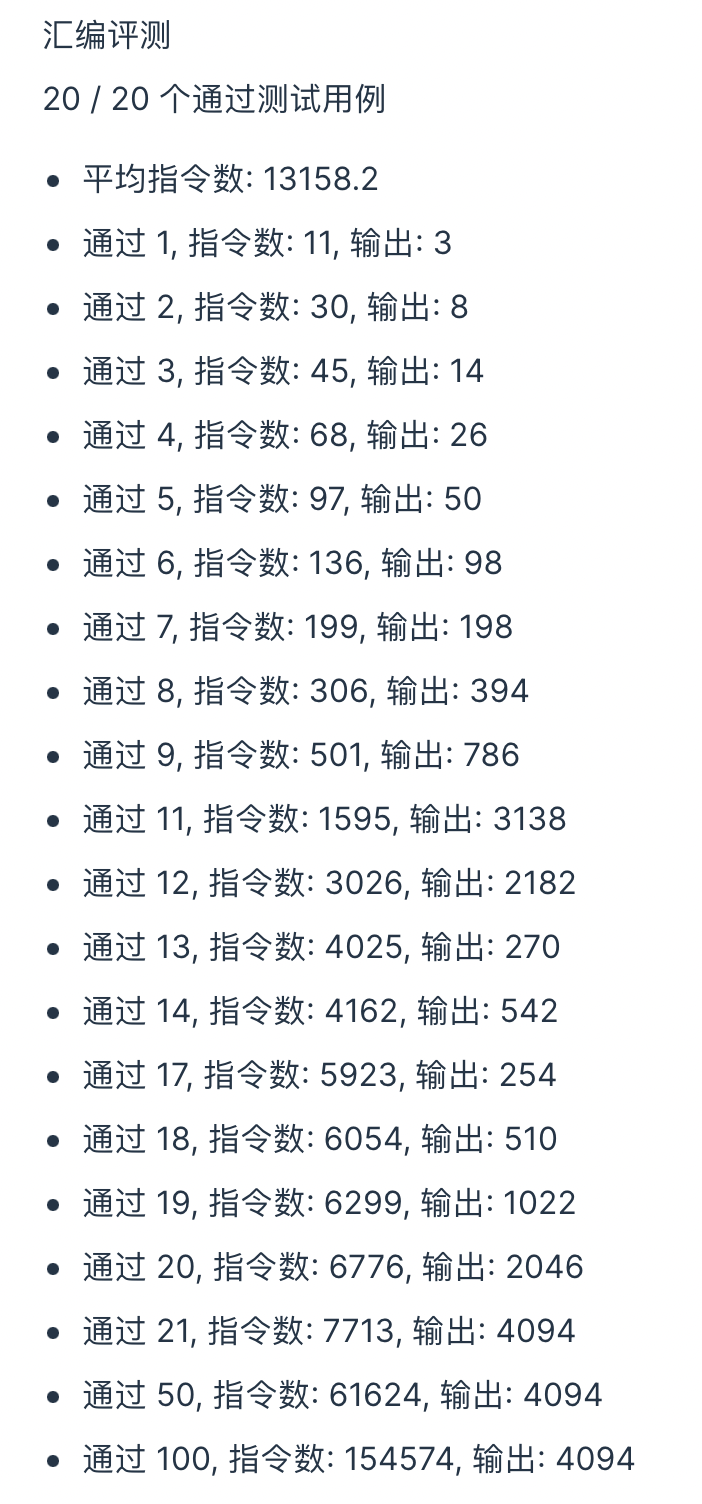
\includegraphics[scale=0.5]{result.png}
        \caption{Result}
\end{figure}

\section{Improvements}
We can improve efficiency by optimizing the checking process. 
As is mentioned above, checking for the last digit requires 
lots of operations when $N$ is big. So a better algorithm
for division might significantly improve efficiency.

One possible approach is to enumerate all possible values of a 16-bit 
binary number from MSB. In this way we can obtain the result within 
$16$ operations.

This approach is not adopted in the program due to limited time and its complexity.

\bibliography{math}

\end{document}
\iffalse
\begin{figure}[H]
    \centering
    \includegraphics[scale=0.5]{name.png}
    \caption{name}
\end{figure}
\fi
